\documentclass[a4paper,11pt,utf8]{scrartcl}

\usepackage[ngerman]{babel}
\usepackage[utf8]{inputenc}
\usepackage[a4paper, left=2cm, right=2cm, top=1.5cm, bottom=1.5cm]{geometry}
\usepackage{graphicx}
\usepackage{stmaryrd}
\usepackage{listings}
\usepackage{amsmath}
\usepackage[hidelinks]{hyperref}
\usepackage[onehalfspacing]{setspace}

\setlength{\headsep}{.5cm}

\begin{document}

\pagestyle{empty}

% Titlepage
\noindent
Praktikum: Big Data \hfill Klemens Schölhorn, Sebastian Lange, Simon Hüning \hfill 30.11.2015\vspace{-.4cm}\\
\begin{center}
\huge\textsf{Lösungsskizze zum ersten Testat}\vspace{.1cm}\\
\large Zitierungsanalyse auf den Daten der DBLP unter Verwendung von Apache Kylin
\end{center}

\section*{Einleitung}

Die ersten drei Abschnitte beschreiben die bisher umgesetzten Arbeiten, während in Sektion \ref{sec:plan} der Plan für die noch ausstehenden Tätigkeiten dargelegt wird.

\section{Server}

\subsection{Software}

Auf dem für das Praktikum zur Verfügung gestellten Rechner \texttt{wdi06} wurde basierend auf dem im installierten Ubuntu 14.04 LTS enthaltenen opendjk-7 folgende Software installiert:

\begin{itemize}
    \item Hadoop (HDFS): 2.7.1
    \item HBase: 0.98.15
    \item Hive: 0.14.0
    \item Kylin: 1.1
    \item Pentaho Data Integration (PDI) -- Community Edition: 6.0
\end{itemize}

\noindent
Es konnten aufgrund von Beschränkungen von Kylin\footnote{\url{http://kylin.incubator.apache.org/docs/install/index.html}} keine aktuellen Versionen von HBase und Hive verwendet werden. Es existiert zwar eine Version von Kylin für HBase 1.1.3, letzteres wurde jedoch noch nicht offiziell veröffentlicht.

\subsection{Einrichtung}

Die Hadoop-Umgebung wurde im pseudo-verteilten Modus installiert, d.\,h. es werden die gleichen Knoten wie in einer verteilten Umgebung verwendet, jedoch alle auf einer physischen Maschine und nur jeweils eine Instanz pro Knotentyp.

Die Installation erfolgte ohne root-Rechte in einem Benutzerverzeichnis durch Setzen der benötigten Umgebungsvariablen (\texttt{HADOOP\_HOME}, \texttt{HBASE\_HOME}, $\dots$). Dabei wurde weitgehend auf die Standard-Konfiguration gesetzt und nur die minimal benötigte Konfiguration vorgenommen.\footnote{Details dazu finden sich im Installationsprotokoll im privaten Repository: \texttt{Installation.txt}}

Da die meisten Dienste standardmäßig an allen Adressen (und damit auch der öffentlichen Adresse) lauschen, wurde zusätzlich die in Ubuntu integrierte Firewall \texttt{ufw} aktiviert.

\section{Datenbankschema}

Das folgende vorläufige Datenbankschema basiert auf dem in der Aufgabenstellung vorgeschlagenen und wurde nur an einigen Stellen geringfügig angepasst. Einige der Schlüssel werden voraussichtlich keine Ganzzahlen, sondern Zeichenketten sein.

\noindent
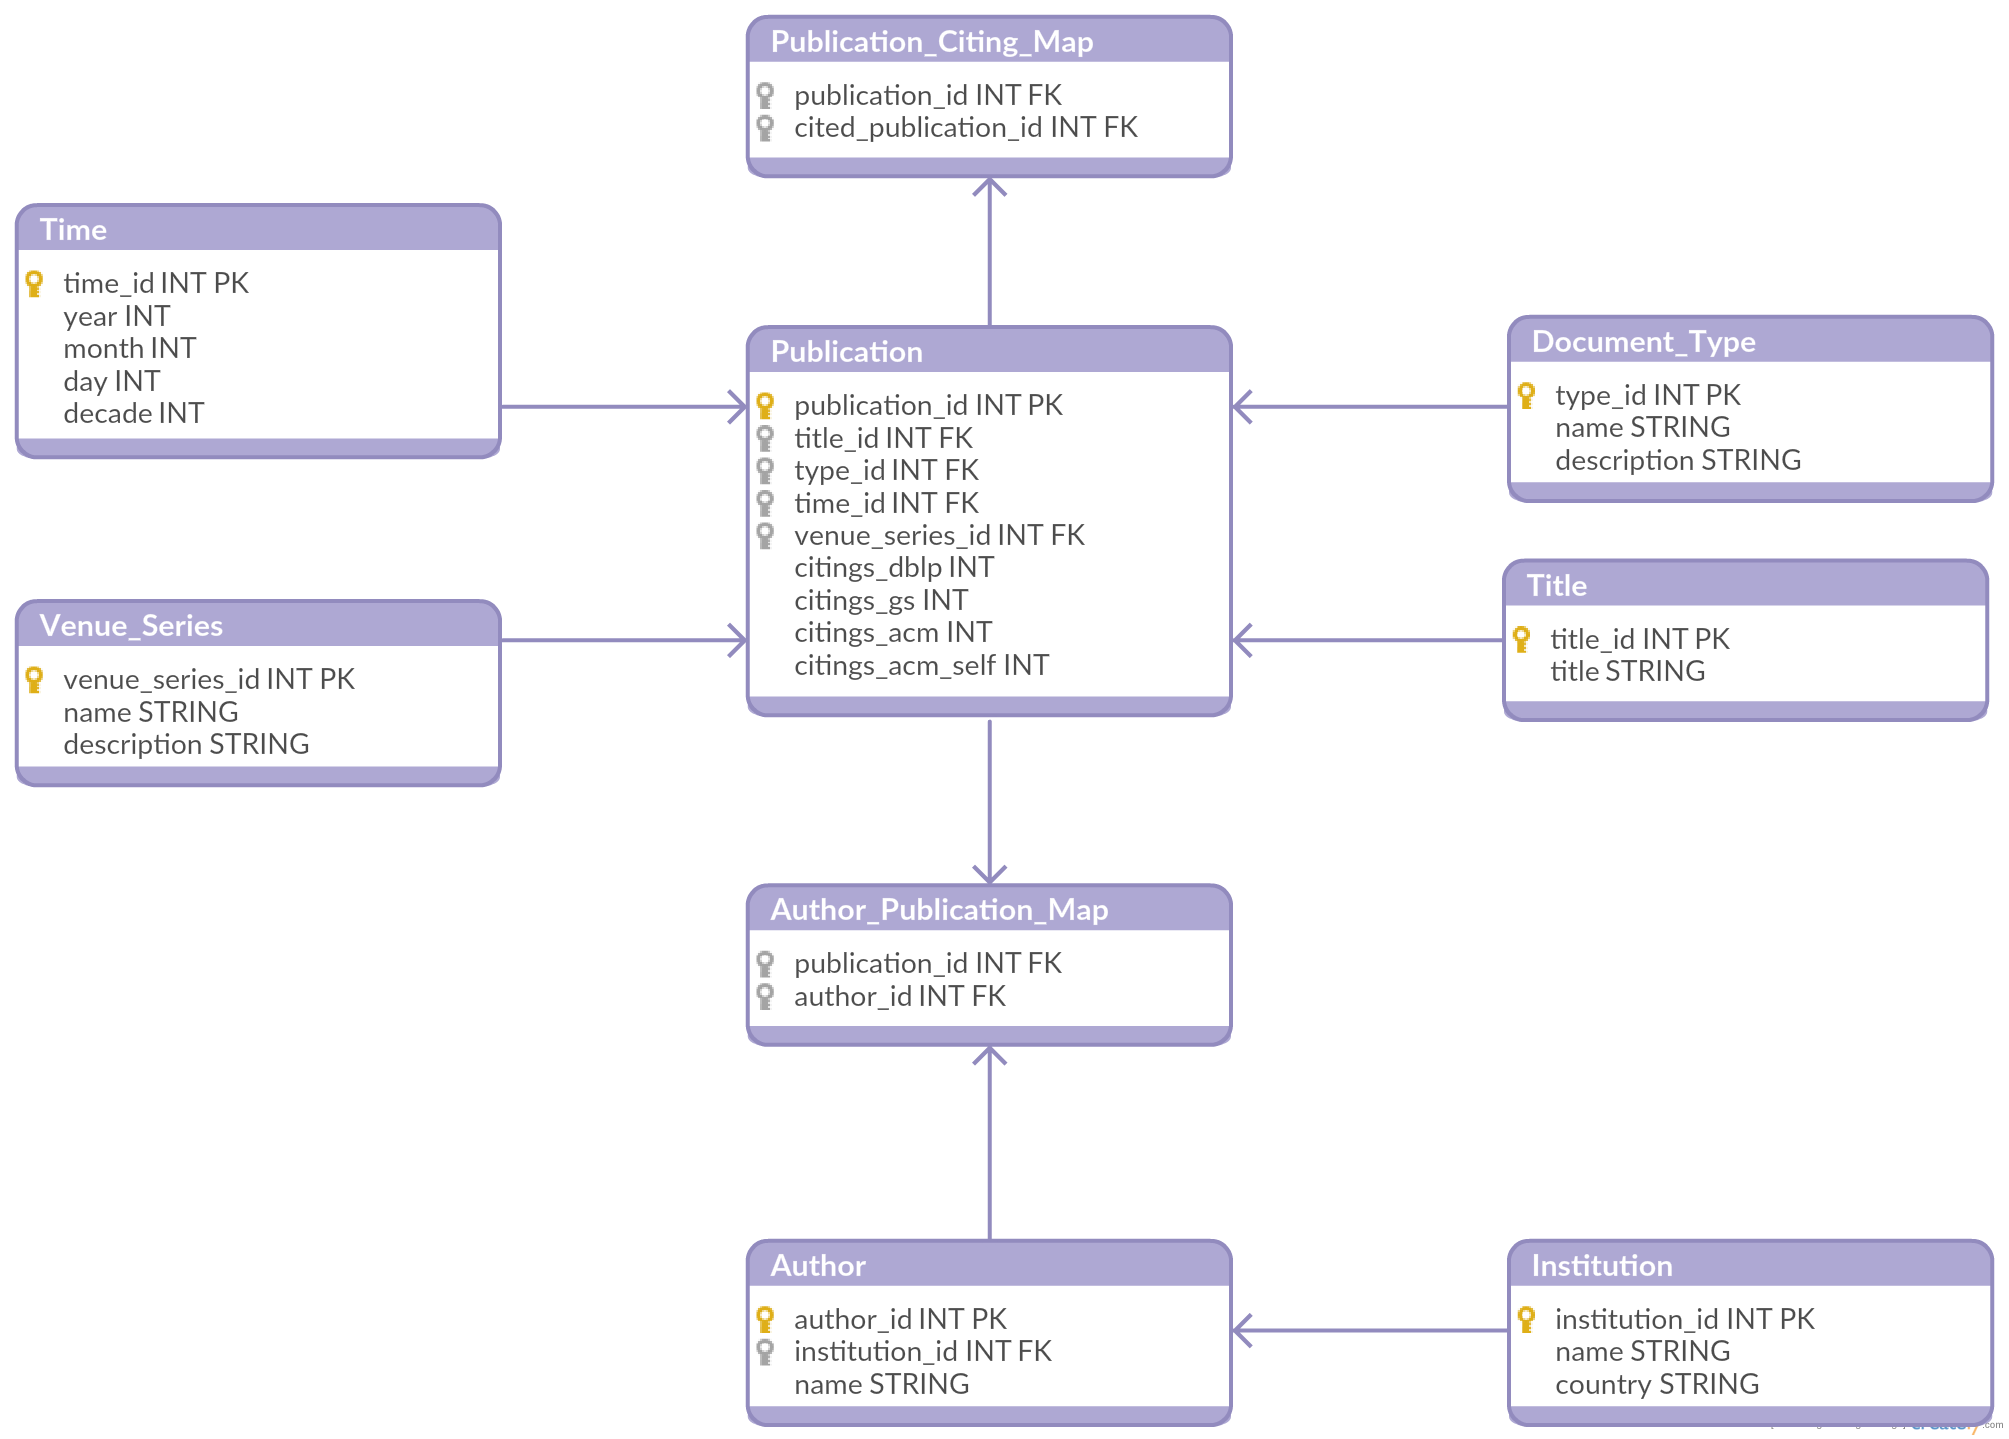
\includegraphics[width=\textwidth]{schema.png}

\begin{itemize}
    \item \texttt{Publication\_Citing\_Map}: Zitat einer Publikation (nicht Teil des endgültigen Sternschemas)
    \item \texttt{Publication}: Zitierungszahlen werden aus \texttt{Publication\_Citing\_Map} generiert
    \item \texttt{Document\_Type}: Typ der Publication, z.\,B. Journal, Artikel, Kollektion
\end{itemize}

\section{Datenimport}

Der Import mit PDI gestaltete sich aufgrund der Datengröße schwierig. So kann die \texttt{dblp.xml} nicht direkt mit einem DOM-Parser verarbeitet werden, da dafür zu viel Speicher benötigt wird. Aus diesem Grund muss ein SAX- oder StaX-Parser verwendet werden, was in Pentaho selbst nur umständlich umzusetzen ist.

Auch ein direkter Import per MapReduce stellte sich als schwierig heraus, da immer komplette XML-Records gelesen werden müssen, was der standardmäßig zeilenweisen Verarbeitung von MapReduce widerspricht. Hadoop besitzt zwar einen \texttt{StreamXmlRecordReader}, der jedoch selbst in aktuellen Versionen scheinbar nicht immer problemlos funktioniert\footnote{\url{https://issues.apache.org/jira/browse/MAPREDUCE-577}}.

Alternativ wird oft \texttt{XmlInputFormat} von Mahout (einem Hadoop-basierten Machine-Learning-Tool) verwendet\footnote{\url{http://oobaloo.co.uk/articles/2010/1/20/processing-xml-in-hadoop.html}}, was diese Probleme nicht hat. Allerdings müssen dabei alle zu lesenden Records das gleiche XML-Tag verwenden, was bei der \texttt{dblp.xml} leider nicht der Fall ist.

Aus diesem Grund haben wir ein eigenes Tool für den Import entwickelt. Der \texttt{dblp-importer}\footnote{\url{https://github.com/klemens/bigdata-kylin-dblp}} liest die \texttt{dblp.xml} aus einer Datei oder von \texttt{stdin}, verwendet StAX für das Parsen und schreibt das Ergebnis anschließend direkt ins HDFS. Dabei ist unabhängig von der Größe der Eingabedatei der Speicherverbrauch konstant.

Die exportierten Daten werden dabei in einem sowohl zu Hive also auch PDI kompatiblen Format geschrieben (CSV mit Backslash als Escape-Zeichen) und bestehen aus zwei Dateien: Einmal die \texttt{Collections} wie Konferenzberichte oder Bücher und schließlich die \texttt{Publications} an sich mit entsprechenden Verweisen auf die \texttt{Collections}.

Die Verarbeitung der CSV-Dateien mit PDI gestaltet sich anschließend deutlich weniger umständlich. Daher erfolgt die Transformation und das Laden der Daten in weitere CSV-Dateien (je Tabelle des Datenschemas eine oder mehrere Dateien) über Transformationen und Jobs in PDI. Hierbei werden die Daten für das DB-Schema passend aufbereitet. Die CSV-Dateien werden wieder direkt in das HDFS geschrieben, sodass auf ihnen direkt externe Tabellen nach obigen Schema definiert werden können. Dieser Transformationsschritt ist momentan nur teilweise implementiert.

\section{Plan}
\label{sec:plan}

\subsection{Verwendung anderer Datenquellen?}

DBLP selbst enthält nicht sehr viele Zitierungen, weshalb erörtert werden sollte, ob zusätzlich noch andere Datenquellen wie z.\,B. ACM verwendet werden sollen. Hierbei wären die Transformationen aus PDI je nach Anforderungen der neuen Datenquellen leicht zu erweitern und bestehende Jobs teilweise wiederverwendbar.

\subsection{Definieren der externen Hive-Tabellen}

Nach Abschluss des Datenverarbeitungsschrittes, bei dem die Daten mit PDI in einzelne CSV-Dateien überführt werden, werden darauf entsprechende externe Hive-Tabellen definiert, um den Zugriff aus Kylin zu ermöglichen. Dies ist aktuell bereits in Arbeit und soll bis Mitte Dezember abgeschlossen werden.  

\subsection{Cube-Generierung mit Kylin}

Wenn die Tabellen in Hive definiert sind, sollte die Generierung der Cubes in Kylin relativ einfach möglich sein. Dies soll bis Ende Dezember erfolgen.

\subsection{Analyse der Daten aus den Cubes}

Nach der Generierung der Cubes sollen darauf u.\,a. die in der Aufgabenstellung beschrieben Abfragen ausgeführt werden. Dies soll bis spätestens 1 Woche vor dem letzten Testat erfolgen.

\end{document}
